\section{ANFIS TSK model}\label{sec:fuzzyanfis}

I'll attempt a different approach for the activity classification: a
Takagi-Sugeno-Kang system tuned using ANFIS.

\subsection{Hyperoptimization of the ANFIS}

First, using the script \code{fishyperopt.m}, I've tried different
configurations for the system by changing the way membership functions are
defined and their number. The script uses the \code{generatefis} stage which,
in turn, uses the MATLAB's functions \code{genfis} and \code{anfis} to generate
and tune the system. The configuration tested are the following:
\begin{itemize}
	\item \code{GridPartitioning} with 4 generalized bell MFs per input;
	\item \code{GridPartitioning} with 4 trapezoidal MFs per input;
	\item \code{GridPartitioning} with 5 generalized bell MFs per input;
	\item \code{GridPartitioning} with 5 trapezoidal MFs per input;
	\item \code{GridPartitioning} with 6 generalized bell MFs per input;
	\item \code{GridPartitioning} with 6 trapezoidal MFs per input;
	\item \code{SubtractiveClustering};
	\item \code{FCMClustering}.
\end{itemize}

Each configuration has been tested with 100 epochs. The one that yielded the
best results is the \code{GridPartitioning} with 6 generalized bell MFs per
input. It achieved a RMSE of \(0.1746\) on the training set and a RMSE of
\(0.1895\) on the test (check) set.

\subsection{ANFIS training}

Finally, using the script \code{fistune.m}, the ANFIS model has been trained
with \(1000\) epochs. Using \(15\%\) of the dataset as test set, it was able to
correctly classify \(97.2\%\) of the samples of the test set and \(98\%\) of
all the samples, as shown in \figref{fig:anfisconfusion}.

\begin{figure}[htbp]
	\centering
	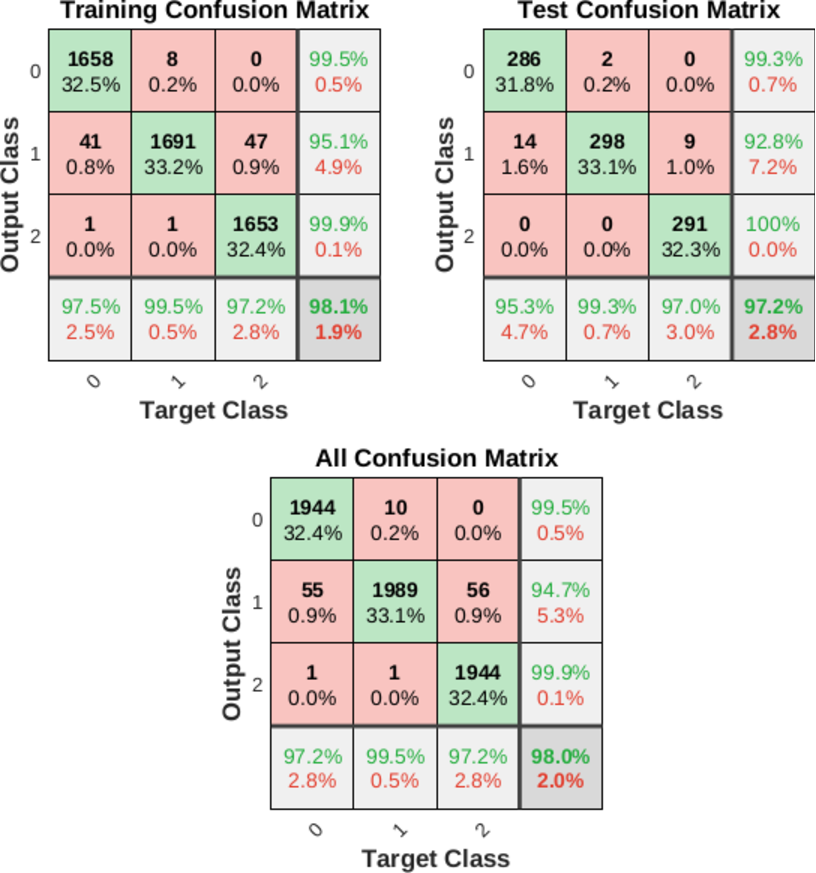
\includegraphics[width=\textwidth]{anfisconfusion}
	\caption{Confusion matrices for the ANFIS TSK
	system.}\label{fig:anfisconfusion}
\end{figure}
